\documentclass[financial_risks_lectures.tex]{subfiles}
\beamertemplatenavigationsymbolsempty

\tikzset{
    invisible/.style={opacity=0,text opacity=0},
    visible on/.style={alt={#1{}{invisible}}},
    alt/.code args={<#1>#2#3}{%
      \alt<#1>{\pgfkeysalso{#2}}{\pgfkeysalso{#3}} % \pgfkeysalso doesn't change the path
    },
  }
\newcommand{\optiontreetimecaption}{	% draw help lines
	%\draw[step=1cm,color=gray] (0,0) grid (16,10);	
	% draw time blocks
	\node [timeblock, text width=1.5cm] (time0) at(1.8,0.5)
		{Сегодня $t=01.10.2014$};
	\node [timeblock, right=3cm of time0, text width=2cm] 			(time1) 
		{1-ый месяц\\$t=$\\01.11.2014};
	\node [timeblock, right=3cm of time1, text width=2.5cm] 		(time2) 
	{2-ой месяц\\$t=$\\01.12.2014};
	% draw time line
	\draw [->](0,1.5) -- (14.5,1.5);	
}  
\newcommand{\drawconnectionarrowspricetree}{    
	\draw [->] (z3-1-1.north east) -- (z1-2-1.west);
    \draw [->] (z3-2-1.south east) -- (z2-2-1.west);
    \draw [->] (z1-1-1.north east) -- (z01-2-1.west);
    \draw [->] (z1-3-1.south east) -- (z02-1-1.north west);
    \draw [->] (z2-1-1.north east) -- (z02-1-1.south west);
    \draw [->] (z2-3-1.south east) -- (z03-1-1.west);
}
\newcommand{\drawconnectionarrowspricetreefortouchoptions}{    
	\draw [->] (z3-1-1.north east) -- (z1-2-1.west);
    \draw [->] (z3-2-1.south east) -- (z2-2-1.west);
    \draw [->] (z1-1-1.north east) -- (z01-2-1.west);
    \draw [->] (z1-2-1.south east) -- (z02-1-1.north west);
    \draw [->] (z2-1-1.north east) -- (z02-1-1.south west);
    \draw [->] (z2-2-1.south east) -- (z03-1-1.west);
}

%\newcommand{\onslidecell}[2]{\onslide<#1->{#2}}
\newcommand{\aheader}[2]{\action<#1-|alert@#1>{#2}}
\subsection{Рыночная волатильность}
\begin{document}
\setbeamercovered{transparent}
\begin{frame}{Биномиальная модель оценки стоимости опционов}
\begin{itemize}[<+->]
\item
Продавец и покупатель всегда имеют противоположные представления о развитии курса товара, лежащего в основе опциона. 
\item
Время в биномиальной модели распределено на периоды, например, дни, недели, месяцы. Курс на начало или конец периода может принимать только два значения: он может либо повысится, либо снизится на определенную процентную величину. 
\item
Биномиальная модель ничего не говорит о вероятности повышения или понижения курса базового актива за период.
\end{itemize}
\end{frame}
\begin{frame}{}
\begin{itemize}[<+->]
\item
Цена опциона в конце срока обращения равна разнице между ценой исполнения и текущей ценой. Причем если получается отрицательная величина, то опцион не исполняется, т.е. его стоимость равна нулю. 
\item
Мы можем, пользуясь математическими параметрами изменения курса, спрогнозировать наиболее вероятный диапазон изменения котировок в течении всего срока обращения опциона. 
\end{itemize}
\end{frame}
\setbeamercovered{invisible}
\begin{frame}[shrink=15]{Изменения котировок USDRUB c 01.10.2013 по 01.10.2014}
\begin{center}
% Table generated by Excel2LaTeX from sheet 'USDRUB'
\begin{table}[htbp]
  \centering
    \begin{tabular}{>{\onslide<1->}c
    				>{\onslide<1->}c        
    				>{\onslide<2->}c}
    \toprule
    \multicolumn{1}{c}{Дата} & \multicolumn{1}{c}{Цена закрытия} & \multicolumn{1}{c}{$\Delta,\%$} \\
    \midrule
    01.10.2013 & 32,0973 &  \\
    01.11.2013 & 33,0852 & 3,08\% \\
    01.12.2013 & 32,8311 & -0,77\% \\
    01.01.2014 & 35,2523 & 7,37\% \\
    01.02.2014 & 35,9238 & 1,90\% \\
    01.03.2014 & 35,1707 & -2,10\% \\
    01.04.2014 & 35,6287 & 1,30\% \\
    01.05.2014 & 34,8855 & -2,09\% \\
    01.06.2014 & 33,9675 & -2,63\% \\
    01.07.2014 & 35,705 & 5,12\% \\
    01.08.2014 & 37,1041 & 3,92\% \\
    01.09.2014 & 39,5562 & 6,61\% \\
    01.10.2014 & 42,9913 & 8,68\% \\
    \bottomrule
    \end{tabular}%
  \label{tab:addlabel}%
\end{table}%
\end{center}
\end{frame}
\begin{frame}{График котировок USDRUB по месяцам}
\begin{center}
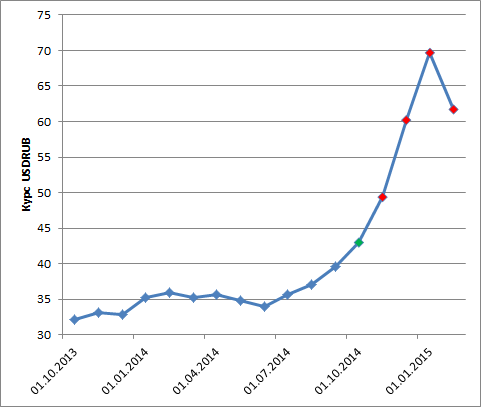
\includegraphics[scale=0.7]{img/usdrubquoteschart}
\end{center}
\end{frame}
\begin{frame}{Процентное изменение котировок USDRUB по месяцам}
\begin{center}
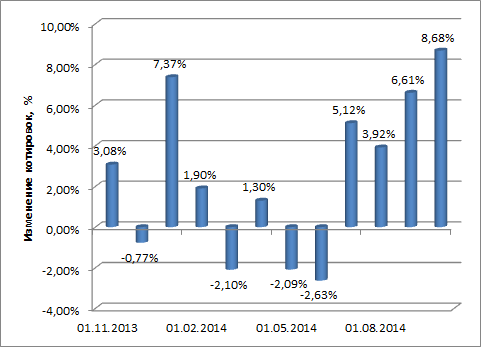
\includegraphics[scale=0.8]{img/usdrubdeltaperc}
\end{center}
\end{frame}
\begin{frame}{Интервалы процентных изменений котировок  USDRUB}
\begin{center}
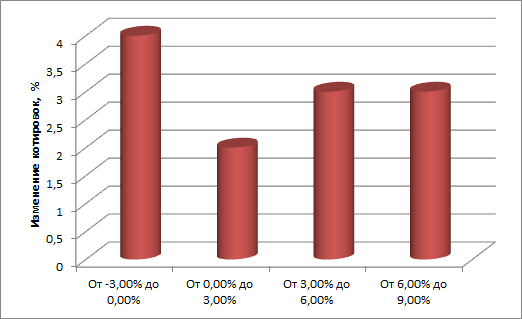
\includegraphics[scale=0.8]{img/usdrubquotesintervals}
\end{center}
\end{frame}
\setbeamercovered{transparent}
\begin{frame}{Формулы для расчета средней и стандартного отклонения}
\begin{itemize}[<+->]
\item
Среднее значение доходности:
$$m=\frac{\sum_{i=1}^n x_i}{n}$$
где $x_i$ – наблюденное значение;

$n$ – количество наблюдений.
\item
Стандартное отклонение:
$$s=\sqrt{\frac{\sum_{i=1}^n (m-x_i)^2}{n-1}}$$
\end{itemize}
\end{frame}
\setbeamercovered{invisible}
\begin{frame}[shrink=15]{Среднее ежемесячное изменение котировок USDRUB и его стандартное отклонение}
% Table generated by Excel2LaTeX from sheet 'Расчет m и s'
\begin{table}[htbp]
  \centering
    \begin{tabular}{cccc}
    \toprule
    & $x_i$    & $m-x_i$  & $(m-x_i)^2$ \\
    \midrule
1 & 3,08\% & \hiddencell{4}{-0,54\%} & \hiddencell{5}{0,30} \\
2 & -0,77\% & \hiddencell{4}{3,30\%} & \hiddencell{5}{10,90} \\
3 & 7,37\% & \hiddencell{4}{-4,84\%} & \hiddencell{5}{23,44} \\
4 & 1,90\% & \hiddencell{4}{0,63\%} & \hiddencell{5}{0,40} \\
5 & -2,10\% & \hiddencell{4}{4,63\%} & \hiddencell{5}{21,44} \\
6 & 1,30\% & \hiddencell{4}{1,23\%} & \hiddencell{5}{1,52} \\
7 & -2,09\% & \hiddencell{4}{4,62\%} & \hiddencell{5}{21,34} \\
8 & -2,63\% & \hiddencell{4}{5,17\%} & \hiddencell{5}{26,68} \\
9 & 5,12\% & \hiddencell{4}{-2,58\%} & \hiddencell{5}{6,66} \\
10 & 3,92\% & \hiddencell{4}{-1,38\%} & \hiddencell{5}{1,92} \\
11 & 6,61\% & \hiddencell{4}{-4,08\%} & \hiddencell{5}{16,61} \\
12 & 8,68\% & \hiddencell{4}{-6,15\%} & \hiddencell{5}{37,83} \\
    \midrule
    $\Sigma$& \hiddencell{2}{30,40\%} 
    &  - 
    & \onslide<6->{169,02} \\
    \textbf{m}
    & \hiddencell{3}{\textit{\textbf{2,5337\%}}} 
    & \textbf{s}
    & \hiddencell{7}{\textit{\textbf{3,9199\%}}} \\
    \bottomrule
    \end{tabular}%
  \label{tab:addlabel}%
\end{table}%

\end{frame}
\begin{frame}{Средняя ежемесячная доходность USDRUB и ее стандартное отклонение}
\begin{center}

% Table generated by Excel2LaTeX from sheet 'Расчет m и s'
\begin{table}[htbp]
  \centering
    \begin{tabular}{lr}
    \toprule
    m     & 2,5337\% \\
    s     & 3,9199\% \\
    \midrule
    m+s   & 6,4535\% \\
    m-s   & -1,3862\% \\
    \midrule
    u     & 1,0645 \\
    d     & 0,9861 \\
    \bottomrule
    \end{tabular}%
  \label{tab:addlabel}%
\end{table}%
\end{center}
\end{frame}
\subsection{Дерево цен}
\begin{frame}{Построение дерева цен}
{Параметры опционов колл и пут}
\begin{center}
% Table generated by Excel2LaTeX from sheet 'Модель'
\begin{table}[htbp]
  \centering
    \begin{tabular}{lrr}
    \toprule
    & \multicolumn{2}{c}{Тип опциона} \\  \cmidrule{2-3}
    & Колл & Пут \\
    \midrule
    Цена исполнения  & 45,00 \rouble & 45,00 \rouble \\
    Срок  & 2 месяца & 2 месяца \\
    Ставка USD, \% год-х & 1\% & 1\% \\
    Ставка RUB, \% год-х & 8,00\% & 8,00\% \\
    Ставка USD, \% мес. & 0,08\% & 0,08\% \\
    Ставка RUB, \% мес. & 0,67\% & 0,67\% \\
    \bottomrule
    \end{tabular}%
  \label{tab:addlabel}%
\end{table}%
\end{center}
\end{frame}
\setbeamercovered{invisible}
\tikzstyle{block} = [rectangle split, 
         rectangle split horizontal, 
         rectangle split parts=2, 
         rectangle split draw splits=true,
         draw, 
		rectangle split part fill={lightgray,white},             minimum height=1.5em, text width=1cm, align=center]

\tikzstyle{timeblock}=[fill=white, rectangle, 
    minimum height=1.5em, minimum width=6em, align=center]

\tikzstyle{tableblock}=[fill=white, rectangle, 
    minimum height=1.5em, minimum width=6em, align=center, draw]

\tikzstyle{optiontreenode}=[space
	,column 1/.style={nodes={cell,minimum width=2em}
	,text width=6.0em}
	,column 2/.style={nodes={cell,minimum width=2em}}]

\tikzstyle{pricetree}=[yscale=-1
,cell/.style={rectangle,draw=black}
,space/.style={matrix of nodes,row sep=-\pgflinewidth,column sep=-\pgflinewidth,column 1/.style={font=\ttfamily}}
,text depth=0.1ex
,text height=1.5ex
,text width=8.5em
,nodes in empty cells
,node distance=0.05cm
,align=right
,background default draw=black % define default behaviour
,background default text=gray!20 % define default behaviour
,background default aspect={solid} % define default behaviour
,highlight/.style={background draw=black% define modified behaviour
,background text=black, % define modified behaviour
,background aspect=solid}% define modified behaviour
]

\begin{frame}[fragile,shrink=35]{Бинарное дерево}
\begin{center}
\begin{tikzpicture}[pricetree]
	\scriptsize
	\optiontreetimecaption
	% draw binary tree model
	\matrix (z3) [optiontreenode] at (2.2,5.3)
	{
	|[fill=gray!20]|42,9913\rouble& $z_3=\trouble$\\
	$x_3=\text{\$}$ & $y_3=\trouble$ \\
	};
	\matrix (z1) [optiontreenode, above right= of z3] 
	{
	& $\alpha=\trouble$\\
	|[highlight, fill=gray!20, text on=<2->]| 45,7658\rouble & $z_1=\trouble$\\
	$x_1=\text{\$}$ & $y_1=\trouble$ \\
	};
	\matrix (z2) [optiontreenode, below right= of z3] 
	{
	|[]|& $\alpha=\trouble$\\
	|[highlight, fill=gray!20, text on=<3->]| 42,3954\rouble & $z_2=\trouble$\\
	$x_2=\text{\$}$ & $y_2=\trouble$ \\
	};
	\matrix (z01) [optiontreenode ,above right= of z1] 
	{
	60,2065\rouble& $z_r=\trouble$ \\
	|[highlight, fill=gray!20, text on=<4->]|48,7193\rouble
	& $z=\trouble$\\
	};
	\matrix (z02) [optiontreenode, above right= of z2] 
	{
	|[highlight, fill=gray!20, text on=<5->]|45,1314\rouble
	& $z=\trouble$\\
	};
	\matrix (z03) [optiontreenode, below right= of z2] 
	{
	|[highlight, fill=gray!20, text on=<6->]|41,8077\rouble
	& $z=\trouble$\\
	};
	% draw connection arrows
	\drawconnectionarrowspricetree
\end{tikzpicture}
\end{center}
\end{frame}

\tikzstyle{optionpricetree}=[yscale=-1
,cell/.style={rectangle,draw=black}
,space/.style={matrix of nodes,row sep=-\pgflinewidth,column sep=-\pgflinewidth,column 1/.style={font=\ttfamily}}
,text depth=0.1ex
,text height=1.5ex
,text width=8.5em
,nodes in empty cells
,node distance=0.05cm
,align=right
,background default draw=black % define default behaviour
,background default text=white % define default behaviour
,background default aspect={solid} % define default behaviour
,highlight/.style={background draw=black% define modified behaviour
,background text=black, % define modified behaviour
,background aspect=solid}% define modified behaviour
]
\begin{frame}[fragile,shrink=35]{Бинарное дерево}
\begin{center}
\begin{tikzpicture}[optionpricetree]
	\scriptsize
	\optiontreetimecaption
	% draw binary tree model
	\matrix (z3) [optiontreenode] at (2.2,5.3)
	{
	|[fill=gray!20]|42,9913\rouble& $z_3=\trouble$\\
	$x_3=\text{\$}$ & $y_3=\trouble$ \\
	};
	\matrix (z1) [optiontreenode, above right= of z3] 
	{
	& $\alpha=\trouble$\\
	|[fill=gray!20]| 45,7658\rouble & $z_1=\trouble$\\
	$x_1=\text{\$}$ & $y_1=\trouble$ \\
	};
	\matrix (z2) [optiontreenode, below right= of z3] 
	{
	|[]|& $\alpha=\trouble$\\
	|[fill=gray!20]| 42,3954\rouble & $z_2=\trouble$\\
	$x_2=\text{\$}$ & $y_2=\trouble$ \\
	};
	\matrix (z01) [optiontreenode ,above right= of z1] 
	{
	60,2065\rouble& $z_r=\trouble$ \\
	|[fill=gray!20]|48,7193\rouble
	& |[highlight, text on=<1->]|$z=3,7193 \trouble$\\
	};
	\matrix (z02) [optiontreenode, above right= of z2] 
	{
	|[fill=gray!20]|45,1314\rouble
	& |[highlight, text on=<2->]| $z=0,1314 \trouble$\\
	};
	\matrix (z03) [optiontreenode, below right= of z2] 
	{
	|[fill=gray!20]|41,8077\rouble
	&|[highlight,text on=<3->]| $z=0\trouble$\\
	};
	% draw connection arrows
	\drawconnectionarrowspricetree
\end{tikzpicture}
\end{center}
\end{frame}
\subsection{Стоимость опциона в промежуточные периоды}
\setbeamercovered{transparent}
\begin{frame}{}
\begin{itemize}[<+->]
\item
Цена опциона в промежуточные периоды определяется путем составления и расчета эквивалентного портфеля. Т.е. портфеля, состоящего из определенного количества базового актива и денег, стоимость которого в любой момент времени равна стоимости опциона на базовый актив.
\item
Зная стоимость опциона на конец рассматриваемого периода и решив систему уравнений мы можем определить стоимость опциона на начало периода и т.д. до дня предполагаемой покупки. Это и будет теоретически справедливая цена опциона.

\end{itemize}
\end{frame}
\begin{frame}{}
\begin{itemize}[<+->]
\item
При расчете стоимости опционов предполагается, что денежная часть эквивалентного портфеля приносит некоторый безрисковый доход, в случае длинной позиции по деньгам (опцион пут) или расход, в случае короткой позиции по деньгам (опцион колл). 
\item
Для расчета принимаем процентную ставку по государственным облигациям США.
\end{itemize}
\end{frame}
\setbeamercovered{invisible}
\begin{frame}[shrink=10]{Пример расчета первой промежуточной цены опциона}
\begin{align*}
\begin{cases} 
\onslide<2->{z_1 = 45,7658 \cdot x_1 + y_1}\\ 
\onslide<3->{3,7193 = 48,7193 \cdot x_1 \cdot (1 + r_{USD}) + y_1 \cdot (1 + r_{RUB})}\\
\onslide<4->{0,1314 = 45,1314 \cdot x_1 \cdot (1 + r_{USD}) + y_1 (1 + \cdot r_{RUB})}
\end{cases}
\end{align*}
$z_1$ – промежуточная цена опциона (искомая величина);

$x_1$ – количество базового актива в портфеле (базовой валюты) отрицательное значение означает короткую позицию;

$y_1$ – количество валюты котировки в портфеле отрицательное значение означает короткую позицию;

$r_{USD},r_{RUB}$ – процентная ставка без риска по займам/депозитам, соответственно, в базовой валюте и валюте котировки, годовых.
\end{frame}
\setbeamercovered{transparent}
\begin{frame}{}
\begin{itemize}[<+->]
\item
При расчетах цены опционов колл и пут используются одинаковые формулы. Различия есть только при определении цены опциона в конце срока обращения (при вычислении  разницы между текущей котировкой базового актива и ценой исполнения опциона).
\item
Промежуточная цена опциона, иногда бывает недостаточно большой, чтобы удержать владельца опциона от его исполнения, в этом случае, в качестве промежуточной цены опциона используется прибыль от его исполнения на рассматриваемую дату.
\end{itemize}
\end{frame}
\setbeamercovered{invisible}
\subsection{Стоимость опциона колл и пут}
\begin{frame}[fragile,shrink=35]{Опцион колл}
\begin{center}
\begin{tikzpicture}[optionpricetree]
	\scriptsize
	\optiontreetimecaption
	% draw binary tree model
	\matrix (z3) [optiontreenode] at (2.2,5.3)
	{
	|[fill=gray!20]|42,9913\rouble
	&|[highlight, text on=<4->]| $z_3=0,2803\trouble$\\
	|[highlight, text on=<4->]|$x_3=\text{\$}0,294$ 
	&|[highlight, text on=<4->]| $y_3=-12,3741\trouble$ \\
	};
	\matrix (z1) [optiontreenode, above right= of z3] 
	{
	&|[highlight, text on=<2->]|$\alpha=0,7658\trouble$\\
	|[fill=gray!20]|45,7658\rouble 
	& |[highlight, text on=<2->]|$z_1=1,0257\trouble$\\
	|[highlight, text on=<2->]| $x_1=\text{\$}0,999$ 
	&|[highlight, text on=<2->]| $y_1=-44,7020\trouble$ \\
	};
	\matrix (z2) [optiontreenode, below right= of z3] 
	{
	&|[highlight, text on=<3->]|$\alpha=0,0000\trouble$\\
	|[fill=gray!20]|42,3954\rouble
	&|[highlight, text on=<3->]|$z_2=0,0328\trouble$\\
	|[highlight, text on=<3->]|$x_2=\text{\$}0,039$ 
	&|[highlight, text on=<3->]|$y_2=-1,6416\trouble$ \\
	};
	\matrix (z01) [optiontreenode ,above right= of z1] 
	{
	60,2065\rouble
	&|[highlight, text on=<5->]|$z_r=15,2065\trouble$ \\
	|[fill=gray!20]|48,7193\rouble
	&$z=3,7193\trouble$\\
	};
	\matrix (z02) [optiontreenode, above right= of z2] 
	{
	|[fill=gray!20]|45,1314\rouble
	&$z=0,1314\trouble$\\
	};
	\matrix (z03) [optiontreenode, below right= of z2] 
	{
	|[fill=gray!20]|41,8077\rouble
	&$z=0,0000\trouble$\\
	};
	% draw connection arrows
    \drawconnectionarrowspricetree
\end{tikzpicture}
\end{center}
\end{frame}
\begin{frame}[fragile,shrink=35]{Опцион пут}
\begin{center}
\begin{tikzpicture}[optionpricetree]
	\scriptsize
	\optiontreetimecaption
	% draw binary tree model
	\matrix (z3) [optiontreenode] at (2.2,5.3)
	{
	|[fill=gray!20]|42,9913\rouble
	&|[highlight, text on=<7->]| $z_3=1.9375\trouble$\\
	|[highlight, text on=<7->]|$x_3=-\text{\$}0.772$ 
	&|[highlight, text on=<7->]| $y_3=35.1334\trouble$ \\
	};
	\matrix (z1) [optiontreenode, above right= of z3] 
	{
	&|[highlight, text on=<5->]|$\alpha=0\trouble$\\
	|[fill=gray!20]|45,7658\rouble 
	& |[highlight, text on=<5->]|$z_1=0\trouble$\\
	|[highlight, text on=<5->]| $x_1=\text{\$}0$ 
	&|[highlight, text on=<5->]| $y_1=0\trouble$ \\
	};
	\matrix (z2) [optiontreenode, below right= of z3] 
	{
	&|[highlight, text on=<6->]|$\alpha=2.6046\trouble$\\
	|[fill=gray!20]|42,3954\rouble
	&|[highlight, text on=<6->]|$z_2=2.6046\trouble$\\
	|[highlight, text on=<6->]|$x_2=-\text{\$}0.960$ 
	&|[highlight, text on=<6->]|$y_2=43.0604\trouble$ \\
	};
	\matrix (z01) [optiontreenode ,above right= of z1] 
	{
	|[fill=gray!20]|48,7193\rouble
	&|[highlight, text on=<2->]|$z=0\trouble$\\
	};
	\matrix (z02) [optiontreenode, above right= of z2] 
	{
	|[fill=gray!20]|45,1314\rouble
	&|[highlight, text on=<3->]|$z=0\trouble$\\
	};
	\matrix (z03) [optiontreenode, below right= of z2] 
	{
	60,2065\rouble
	&|[highlight, text on=<8->]|$z_r=0\trouble$ \\
	|[fill=gray!20]|41,8077\rouble
	&|[highlight, text on=<4->]|$z=3.1923\trouble$\\
	};
	% draw connection arrows
    \drawconnectionarrowspricetree
\end{tikzpicture}
\end{center}
\end{frame}
\subsection{Стоимость бинарных опционов}
\begin{frame}{Стоимость бинарных опционов}
{Параметры бинарных опционов}
\begin{center}

% Table generated by Excel2LaTeX from sheet 'Модель'
\begin{table}[htbp]
  \centering
    \begin{tabular}{lrr}
    \toprule
    & \multicolumn{2}{c}{Тип опциона} \\  \cmidrule{2-3}
    & 1 касание & б/ касаний \\
    \midrule
    Барьерная цена & 48,00 \rouble & 42,50 \rouble \\
    Выплата & \$1 000 & \$1 000 \\
    Срок  & 2 месяца & 2 месяца \\
    Ставка USD, \% год-х & 1\% & 1\% \\
    Ставка RUB, \% год-х & 8,00\% & 8,00\% \\
    Ставка USD, \% мес. & 0,08\% & 0,08\% \\
    Ставка RUB, \% мес. & 0,67\% & 0,67\% \\
    \bottomrule
    \end{tabular}%
  \label{tab:addlabel}%
\end{table}%
\end{center}
\end{frame}
\begin{frame}[fragile,shrink=35]{Опцион в одно касание}
\begin{center}
\begin{tikzpicture}[optionpricetree]
	\scriptsize
	\optiontreetimecaption
	% draw binary tree model
	\matrix (z3) [optiontreenode] at (2.2,5.3)
	{
	|[fill=gray!20]|42,9913\rouble
	&|[highlight, text on=<7->]| $z_3=\text{\$}62$\\
	|[highlight, text on=<7->]|$x_3=\text{\$}3179$ 
	&|[highlight, text on=<7->]| $y_3=-134028\trouble$ \\
	};
	\matrix (z1) [optiontreenode, above right= of z3] 
	{
	|[fill=gray!20]|45,7658\rouble 
	& |[highlight, text on=<5->]|$z_1=\text{\$}249$\\
	|[highlight, text on=<5->]| $x_1=\text{\$}12745$ 
	&|[highlight, text on=<5->]| $y_1=-571865\trouble$ \\
	};
	\matrix (z2) [optiontreenode, below right= of z3] 
	{
	|[fill=gray!20]|42,3954\rouble
	&|[highlight, text on=<6->]|$z_2=\text{\$}0$\\
	|[highlight, text on=<6->]|$x_2=\text{\$}0$ 
	&|[highlight, text on=<6->]|$y_2=0\trouble$ \\
	};
	\matrix (z01) [optiontreenode ,above right= of z1] 
	{
	60,2065\rouble
	&|[highlight, text on=<8->]|$z_r=\text{\$}1000$ \\
	|[fill=gray!20]|48,7193\rouble
	&|[highlight, text on=<2->]|$z=\text{\$}1000$\\
	};
	\matrix (z02) [optiontreenode, above right= of z2] 
	{
	|[fill=gray!20]|45,1314\rouble
	&|[highlight, text on=<3->]|$z=\text{\$}0$\\
	};
	\matrix (z03) [optiontreenode, below right= of z2] 
	{
	|[fill=gray!20]|41,8077\rouble
	&|[highlight, text on=<4->]|$z=\text{\$}0$\\
	};
	% draw connection arrows
    \drawconnectionarrowspricetreefortouchoptions
\end{tikzpicture}
\end{center}
\end{frame}
\begin{frame}[fragile,shrink=35]{Опцион без касаний}
\begin{center}
\begin{tikzpicture}[optionpricetree]
	\scriptsize
	\optiontreetimecaption
	% draw time line
	\draw [->](0,1.5) -- (14.5,1.5);	
	% draw binary tree model
	\matrix (z3) [optiontreenode] at (2.2,5.3)
	{
	|[fill=gray!20]|42,9913\rouble
	&|[highlight, text on=<7->]| $z_3=\text{\$}249$\\
	|[highlight, text on=<7->]|$x_3=\text{\$}12745$ 
	&|[highlight, text on=<7->]| $y_3=-537197\trouble$ \\
	};
	\matrix (z1) [optiontreenode, above right= of z3] 
	{
	|[fill=gray!20]|45,7658\rouble 
	& |[highlight, text on=<5->]|$z_1=\text{\$}1000$\\
	|[highlight, text on=<5->]| $x_1=\text{\$}1000$ 
	&|[highlight, text on=<5->]| $y_1=-45766\trouble$ \\
	};
	\matrix (z2) [optiontreenode, below right= of z3] 
	{
	|[fill=gray!20]|42,3954\rouble
	&|[highlight, text on=<6->]|$z_2=\text{\$}0$\\
	|[highlight, text on=<6->]|$x_2=\text{\$}0$ 
	&|[highlight, text on=<6->]|$y_2=0\trouble$ \\
	};
	\matrix (z01) [optiontreenode ,above right= of z1] 
	{
	60,2065\rouble
	&|[highlight, text on=<8->]|$z_r=\text{\$}1000$ \\
	|[fill=gray!20]|48,7193\rouble
	&|[highlight, text on=<2->]|$z=\text{\$}1000$\\
	};
	\matrix (z02) [optiontreenode, above right= of z2] 
	{
	|[fill=gray!20]|45,1314\rouble
	&|[highlight, text on=<3->]|$z=\text{\$}0$\\
	};
	\matrix (z03) [optiontreenode, below right= of z2] 
	{
	|[fill=gray!20]|41,8077\rouble
	&|[highlight, text on=<4->]|$z=\text{\$}0$\\
	};
	% draw connection arrows
    \drawconnectionarrowspricetreefortouchoptions
\end{tikzpicture}
\end{center}
\end{frame}
\setbeamercovered{transparent}
\subsection{Общая однопериодная модель}
\begin{frame}[shrink=15]{Общая однопериодная модель}
\begin{center}
\begin{tikzpicture}[auto, node distance=0.3cm,>=latex']
	\scriptsize
    \node [block] (sc) {$S$ \nodepart{two} $C$}; 
	\node [block, above right=of sc, node distance=0.3cm] (uS) {$u \cdot S$ \nodepart{two} $C_u$};       
	\node [block, below right=of sc, node distance=0.3cm] (dS) {$d \cdot S$ \nodepart{two} $C_d$};       
	\node [block, above right=of uS, node distance=0.3cm, text width=1.3cm] (definitions) {Валютный курс \nodepart{two} Цена опциона};       
	\node [timeblock, left=of definitions, node distance=0.3cm, text width=2cm] (time1) {Момент окончания $t=T$};
	\node [timeblock, left=0.8cm of time1, text width=1.5cm] (time0) {Момент начала $t=0$};

    \draw [-] (sc) -- (uS);
    \draw [-] (sc) -- (dS);
\end{tikzpicture}
\end{center}
где
$S$ - текущая цена базового актива;

$E$ - цена исполнения опциона.
\begin{align}
C_u = \begin{cases} u \cdot S - E, & \mbox{для случая } u \cdot S > E \\ 
0, & \mbox{для случая } u \cdot S \leq E \end{cases}\\
C_d = \begin{cases} d \cdot S - E, & \mbox{для случая } d \cdot S > E \\ 
0, & \mbox{для случая } d \cdot S \leq E \end{cases}
\end{align}
\end{frame}
\begin{frame}[shrink=15]{Система уравнений\\для однопериодной модели}{и ее решение}
\begin{align}
\begin{cases} 
C = S \cdot x + y\\ 
C_u = u \cdot S \cdot x \cdot r_{USD} + y \cdot r_{RUB}\\
C_d = d \cdot S \cdot x \cdot r_{USD} + y \cdot r_{RUB}
\end{cases}\\[12pt]
x=\frac{C_u-C_d}{(u-d)\cdot S \cdot r_{USD}}
y=\frac{u \cdot C_d-d \cdot C_u}{(u-d) \cdot r_{RUB}}
\end{align}
\begin{align}
C = S \cdot x + y
\end{align}

где

$x, y$ - размеры позиций, соответственно, в долларах и рублях;

$r_{USD},r_{RUB}$ - процентные ставки по заимствованию (кредитованию) за период времени \textit{T}, соответственно, в долларах и рублях.
\end{frame}


\end{document}